% inclui métricas
% introduçao ao gerenciamento de projetos de software
\lecturetitle{\course}{Gerenciamento de Projetos}

\frame{\maketitle}

\begin{frame}{Análise da viabilidade}
  \begin{itemize}[<+-| alert@+>]
  \item {\bf Técnica:} Levantamento dos requisitos técnicos do projeto e
    verificação dos riscos envolvidos na execução baseada na
    capacidade técnica da equipe.
  \item {\bf Operacional:} Verificação de alternativas viáveis e prontas de
    terceiros como solução para a requisição de software.
  \item {\bf Econômica:} Estimativa do custo operacional. (A grande
    dificuldade é a natureza abstrata do software)
  \end{itemize}
\end{frame}

\begin{frame}{Etapas}
  \begin{itemize}[<+-| alert@+>]
  \item Elaboração da proposta;
  \item Planejamento e desenvolvimento do cronograma do projeto;
  \item Levantamento de custo;
  \item Monitoramento e revisões do projeto;
  \item Seleção e avaliação de pessoal;
  \item Elaboração de relatórios e apresentações.
  \end{itemize}
\end{frame}

\begin{frame}{Cronograma}
  Exemplo de diagrama Gantt.\\
  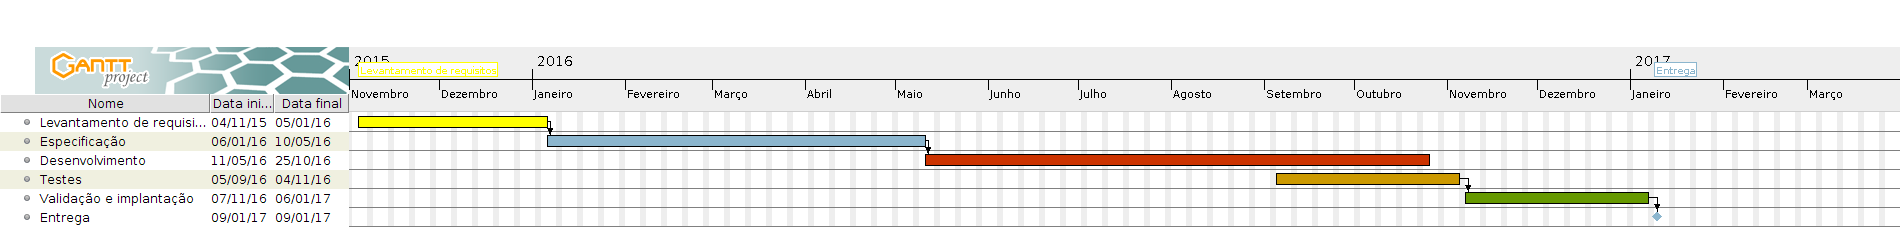
\includegraphics[scale=.19]{img/exemplo-gantt.png}
\end{frame}

\begin{frame}{Alocação de pessoas}
  Exemplo de diagrama Gantt para alocação de pessoas.\\
  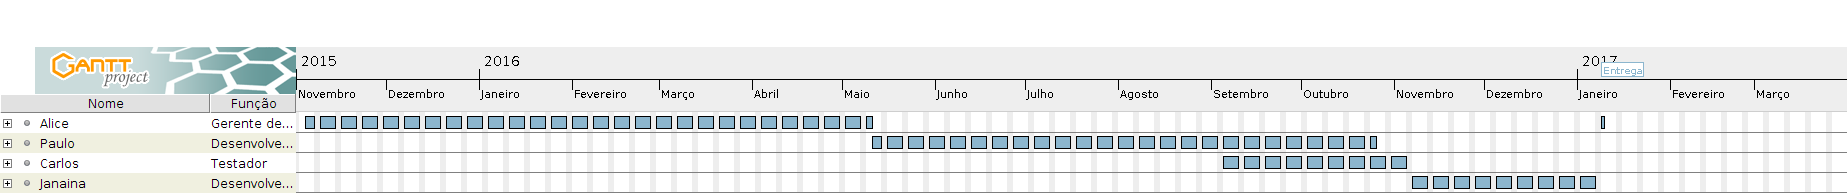
\includegraphics[scale=.19]{img/exemplo-ganttp.png}
\end{frame}

\begin{frame}{Diagrama PERT}{Ordenação topológica}
\begin{center}
  Exemplo de diagrama PERT.\\\bigskip
  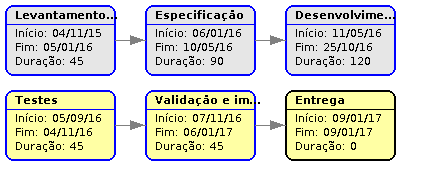
\includegraphics[scale=.4]{img/exemplo-gantt-pert.png}
\end{center}
\end{frame}


% \begin{frame}{Análise de custo}
%   \begin{itemize}
%   \item {\bf Pessoal:} analista, desenvolvedores, gestores, suporte,
%     $\ldots$;
%   \item {\bf Equipamentos:} hardware, impressoras, scanners, $\ldots$;
%   \item {\bf Despesas gerais:} alugueis, serviços externos,
%     treinamento, energia, $\ldots$
%   \end{itemize}
% \end{frame}

\begin{frame}{Ferramentas}
  \begin{itemize}[<+-| alert@+>]
  \item
    \href{https://products.office.com/pt-br/project/project-and-portfolio-management-software}{Microsoft
      Project}: ferramenta completa para gerenciamento de projetos,
    permite a colaboração entre os integrantes do projeto e possui
    integração com planilhas e documentos gerados por produtos da
    Microsoft.
  \item \href{http://www.projectlibre.org/}{ProjectLibre}: alternativa
    gratuita ao Microsoft Project, busca implementar os mesmos
    recursos.
  \item \href{https://www.openproject.org/}{OpenProject}: ferramenta livre baseada 
    na web.
  \item \href{http://www.ganttproject.biz/}{GanttProject}: suporte a
    gráficos Gantt, restrições de dependência e marcos ({\it milestones}).
  \item \href{http://www.taskjuggler.org/}{TaskJuggler}: ferramenta
    flexivel e poderosa para gerenciamento de projetos.
  \end{itemize}
\end{frame}

\begin{frame}{Referências}
  \begin{itemize}
  \item \ianref{}
  \item \ariadneref{}
  \end{itemize}
\end{frame}